\section{Kaka Kamaludin (1174067)}
\subsection{Menulis Shapefile dengan PySHP}
\begin{enumerate}
	\item Jawaban Nomor 1
	\lstinputlisting{src/tugas2/1174067/1.py}
	\begin{figure}[H]
		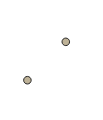
\includegraphics[width=6cm]{figures/Tugas2/1174067/1.png}
		\centering
		\caption{Point (Titik)}
	\end{figure}
	\item Jawaban Nomor 2
	\lstinputlisting{src/tugas2/1174067/2.py}
	\begin{figure}[H]
		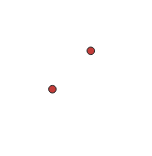
\includegraphics[width=6cm]{figures/Tugas2/1174067/2.png}
		\centering
		\caption{Point (Titik)}
	\end{figure}
	\item Jawaban Nomor 3
	\lstinputlisting{src/tugas2/1174067/3.py}
	\begin{figure}[H]
		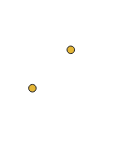
\includegraphics[width=6cm]{figures/Tugas2/1174067/3.png}
		\centering
		\caption{Point (Titik)}
	\end{figure}
	\item Jawaban Nomor 4
	\lstinputlisting{src/tugas2/1174067/4.py}
	\begin{figure}[H]
		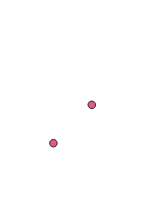
\includegraphics[width=6cm]{figures/Tugas2/1174067/4.png}
		\centering
		\caption{Point (Titik)}
	\end{figure}
	\item Jawaban Nomor 5
	\lstinputlisting{src/tugas2/1174067/5.py}
	\begin{figure}[H]
		
\includegraphics[width=6cm]{figures/Tugas2/1174067/5.png}
		\centering
		\caption{PolyLine (Garis)}
	\end{figure}
	\item Jawaban Nomor 6
	\lstinputlisting{src/tugas2/1174067/6.py}
	\begin{figure}[H]
		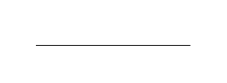
\includegraphics[width=6cm]{figures/Tugas2/1174067/6.png}
		\centering
		\caption{Polygon (Bidang)}
	\end{figure}
	\item Jawaban Nomor 7
	\lstinputlisting{src/tugas2/1174067/7.py}
	\begin{figure}[H]
		
\includegraphics[width=6cm]{figures/Tugas2/1174067/7.png}
		\centering
		\caption{Polygon (Bidang)}
	\end{figure}
	\item Jawaban Nomor 8
	\lstinputlisting{src/tugas2/1174067/8.py}
	\begin{figure}[H]
		
\includegraphics[width=6cm]{figures/Tugas2/1174067/8.png}
		\centering
		\caption{Polygon (Bidang)}
	\end{figure}
	\item Jawaban Nomor 9
	\lstinputlisting{src/tugas2/1174067/9.py}
	\begin{figure}[H]
		
\includegraphics[width=6cm]{figures/Tugas2/1174067/9.png}
		\centering
		\caption{Polygon (Bidang)}
	\end{figure}
	\item Jawaban Nomor 10
	\lstinputlisting{src/tugas2/1174067/10.py}
	\begin{figure}[H]
		
\includegraphics[width=6cm]{figures/Tugas2/1174067/10.png}
		\centering
		\caption{Polygon, Hasil modulus 8 dari npm 1174067 adalah 3 sesui nomor 3 bidang persegipanjang dan angka akhir dari npm saya adalah 6 jadi membuat bidangnya sebanyak 6}
	\end{figure}
\end{enumerate}
\subsection{Link}
	https://youtu.be/URpORX8dxAo